\chapter{Formal Concept Analysis}
\label{chapter:formal-concept-analysis}

Formal Concept Analysis (FCA) provides a simple, and yet mathematically rigorous, framework for identifying and reasoning about ``concepts'' and their corresponding hierarchies in data \cite{ganter1999formal,ganter2016conceptual}. The central view of concepts as a dual between \textit{extension}---what one refers to as instances of a concept---and \textit{intension}---what meaning is ascribed to a concept---is supported by a rich philosophical backing. \index{formal concept analysis} \index{extension} \index{intension}

\section{Basic Notions}
\label{section:basic-notions}
The universe of discourse in FCA is made-up of sets of \textit{objects} and \textit{attributes}. Objects are extensional, they are the things pointed to as instances of some more general concept. In turn, attributes construct the intensional component of a concept.

We collect these extensional and intensional building blocks in a structure called a \textit{formal context}, which includes a binary relation that allows traversal from extension to intension, and vice verse.

\begin{definition}
  \label{definition:formal-context}
  A \textit{formal context} $\Fcontext$ is a triple comprised of a set of objects $G$, a set of attributes $M$, and a binary relation $I \subseteq G \times M$ referred to as an `incidence' relation. For an object-attribute pair $(g,m) \in I$ we might say that \say{object $g$ \textit{has} the attribute $m$}.
\end{definition}

A formal context \index{formal context} in some sense describes an open-world interpretation, and so $(g,m) \not \in I$ is not usually interpreted as saying that \say{object $g$ has the negation of the attribute $m$}.

\begin{example}
  \label{example:first-example-formal-context}
  Finite formal contexts of a reasonable size can be described entirely by a tabular representation. Each object corresponds to a row, and each attribute to a column.

  \begin{figure}[H]
    \centering
    \scriptsize
    \begin{tabular}{|c||c|c|c|c|c|}
      \hline
      & \rotatebox{0}{\texttt{closure}}
      & \rotatebox{0}{\texttt{associativity}}
      & \rotatebox{0}{\texttt{identity}}
      & \rotatebox{0}{\texttt{divisibility}}
      & \rotatebox{0}{\texttt{commutativity}} \\
      \hline\hline
      \texttt{magma}             & $\times$ &          &          &          &          \\ \hline
      \texttt{semigroup}         & $\times$ & $\times$ &          &          &          \\ \hline
      \texttt{monoid}            & $\times$ & $\times$ & $\times$ &          &          \\ \hline
      \texttt{group}             & $\times$ & $\times$ & $\times$ & $\times$ &          \\ \hline
      \texttt{abelian group}     & $\times$ & $\times$ & $\times$ & $\times$ & $\times$ \\ \hline
      \texttt{loop}              & $\times$ &          & $\times$ & $\times$ &          \\ \hline
      \texttt{quasigroup}        & $\times$ &          &          & $\times$ &          \\ \hline
      \texttt{groupoid}          &          & $\times$ & $\times$ & $\times$ &          \\ \hline
      \texttt{category}          &          & $\times$ & $\times$ &          &          \\ \hline
      \texttt{semicategory}      &          & $\times$ &          &          &          \\ \hline
      \specialrule{1.25pt}{0pt}{0pt}
    \end{tabular}
    \caption{A formal context showing necessary properties of group-like structures.}
    \label{figure:formal-context-group-structures}
  \end{figure}
\end{example}

The tabular representation of a formal context allows for easy identification of the set of attributes that a given object satisfies: one need only scan across the respective row in the table and note where an `$\times$' symbol appears. This set of attributes is called the \textit{object intent}. The dual notion of an \textit{attribute extent} can similarly be found by scanning down the column of a given attribute. The utility of this visual metaphor diminishes when, as is often the case, we consider larger sets of objects or attributes. Instead, we opt for a more formal approach to determining the intents and extents for (sets of) objects and attributes, respectively. \index{derivation operators! object intent} \index{derivation operators! attribute extent}

\begin{definition}
  \label{definition:derivation-operators}
  Given a formal context $\fcontext$, the \textit{derivation operators} are two order-reversing maps $(\cdot)^\uparrow : 2^G \to 2^M$ and $(\cdot)^\downarrow : 2^M \to 2^G$ where the order is given by subset inclusion. Then, for any subsets $A \subseteq G$ and $B \subseteq M$,
  \begin{align*}
    A^\uparrow \coloneqq \{m \in M \mid \forall g \in A, \; \langle g,m \rangle \in I\} \\
    B^\downarrow \coloneqq \{g \in G \mid \forall m \in B, \; \langle g,m \rangle \in I\}
  \end{align*}
\end{definition}

The derivation operators provide a clear way of describing, for a given set $A\subseteq G$ of objects, the set of attributes which every object in $A$ satisfies, denoted $A^\uparrow$. As an illustration, given the set of objects $\{\texttt{semigroup, monoid}\}$ from \Cref{figure:formal-context-group-structures}, its derivation would be $\{\texttt{closure, associativity}\}$. It is quite easy to spot that this is just the intersection of the object intents of \texttt{semigroup} and \texttt{monoid}.

Of course, these two functions can be composed; and so, $A^{\uparrow \downarrow}$ would yield the set of objects 

$\{\texttt{semigroup, monoid, group, abelian group}\}$, which can rather cumbersomely be described as ``the set of all  objects that satisfy all the attributes satisfied by \texttt{semigroup} and \texttt{monoid}''.

% If we were to then take the derivation of this set of attributes, $A^{\uparrow \downarrow}$, we get the set of objects $\{\texttt{semigroup, monoid, group, abelian group}\}$: the set of all group-likes that have a closed and associative binary operation!

In fact, this double-application of derivation operators satisfies very specific properties,
\begin{align}
  & \text{(monotonicity)} & A \subseteq A_1 \textit{ implies } A^{\uparrow \downarrow} \subseteq A_1^{\uparrow \downarrow} \\
  & \text{(extensivity)}  & A \subseteq A^{\uparrow \downarrow} \\
  & \text{(idempotency)}  & A^{\uparrow \downarrow} = (A^{\uparrow \downarrow})^{\uparrow \downarrow}
\end{align}
for all $A, A_1 \subseteq G$. Thus, $(\cdot)^{\uparrow \downarrow}$ describes a closure operator on $2^G$. The dual notion holds for attributes, and $(\cdot)^{\downarrow \uparrow}$ describes a closure operator on $2^M$.

\begin{proposition}
  \label{proposition:properties-about-derivation-operators}
  Let $\fcontext$ be a formal context with subsets $A_0, A_1, A_2 \subseteq G$ and $B_0, B_1, B_2 \subseteq M$ of attributes. Then,
  \begin{center}
    \begin{minipage}[t]{0.48\textwidth}
      \begin{enumerate}
        \item $A_0 \subseteq A_1 \Rightarrow A_1^\uparrow \subseteq A_0^\uparrow$
        \item $A_0 \subseteq A_0^{\uparrow \downarrow}$
        \item $A_0^\uparrow = A_0^{\uparrow \downarrow \uparrow}$
      \end{enumerate}
    \end{minipage}%
    \hfill
    \begin{minipage}[t]{0.48\textwidth}
      \begin{enumerate}
        \item $B_0 \subseteq B_1 \Rightarrow B_1^\downarrow \subseteq B_0^\downarrow$
        \item $B_0 \subseteq B_0^{\downarrow \uparrow}$
        \item $B_0^\downarrow = B_0^{\downarrow \uparrow \downarrow}$
      \end{enumerate}
    \end{minipage}
  \end{center}
\end{proposition}

\begin{definition}
  \label{definition:formal-concept}
  A \textit{formal concept} of a formal context $\fcontext$ is a pair $(A,B)$ of subsets $A \subseteq G$ and $B \subseteq M$ that satisfies $A^\uparrow = B$ and $B^\downarrow = A$. Then, $A$ is the concept \textit{extent} and $B$ is the \textit{intent}. We write $\B$ to denote the set of all concepts of $\fcontext$.
\end{definition}
\index{formal concept}

Now explain why derivation of set of objects is always a concept intent by proposition 1. And the dual. and Galois connections
\index{Galois connections}

\begin{figure}[H]
  \centering
  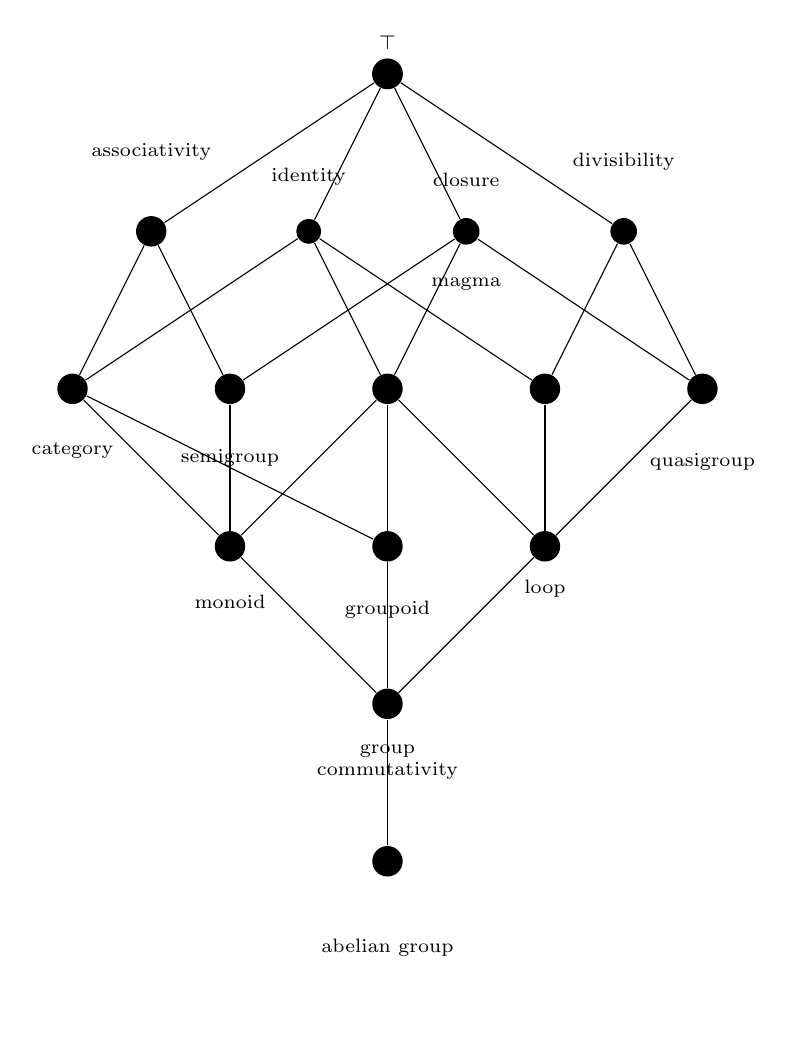
\begin{tikzpicture}[every node/.style={circle, fill=black, inner sep=1pt}]
    \node (a1) at (0,3) [label=above:{\scriptsize $\top$}] {w};
    % \node[draw=none, fill=none] at (0,3.5) {\tiny Top};

    \node (b1) at (-3,1) [label=above:{\scriptsize associativity}] {y};
    \draw (a1) -- (b1);

    \node (b2) at (-1,1) [label=above:{\scriptsize identity}] {z};
    \draw (a1) -- (b2);

    \node (b3) at (1,1) [label=above:{\scriptsize closure},label=below:{\scriptsize magma}] {x};
    \draw (a1) -- (b3);

    \node (b4) at (3,1) [label=above:{\scriptsize divisibility}] {x};
    \draw (a1) -- (b4);

    \node (c1) at (-4,-1) [label=below:{\scriptsize category}] {y};
    \draw (c1) -- (b1);
    \draw (c1) -- (b2);

    \node (c2) at (-2,-1) [label=below:{\scriptsize semigroup}] {y};
    \draw (c2) -- (b1);
    \draw (c2) -- (b3);

    \node (c3) at (0,-1) {y};
    \draw (c3) -- (b2);
    \draw (c3) -- (b3);

    \node (c4) at (2,-1) {y};
    \draw (c4) -- (b2);
    \draw (c4) -- (b4);

    \node (c5) at (4,-1) [label=below:{\scriptsize quasigroup}] {y};
    \draw (c5) -- (b3);
    \draw (c5) -- (b4);

    \node (d1) at (-2,-3) [label=below:{\scriptsize monoid}] {y};
    \draw (d1) -- (c1);
    \draw (d1) -- (c2);
    \draw (d1) -- (c3);

    \node (d2) at (0,-3) [label=below:{\scriptsize groupoid}] {y};
    \draw (d2) -- (c1);
    \draw (d2) -- (c3);

    \node (d3) at (2,-3) [label=below:{\scriptsize loop}] {y};
    \draw (d3) -- (c3);
    \draw (d3) -- (c4);
    \draw (d3) -- (c5);

    \node (e1) at (0,-5) [label=below:{\scriptsize group}] {y};
    \draw (e1) -- (d1);
    \draw (e1) -- (d2);
    \draw (e1) -- (d3);

    \node (f1) at (0,-7)[label=above:{\scriptsize commutativity},label=below:{\scriptsize abelian group}] {y};
    \draw (f1) -- (e1);
  \end{tikzpicture}
  \caption{The concept lattice associated with the formal context in \Cref{figure:formal-context-group-structures}}
\end{figure}

